\chapter{Theoretical Background}
\label{cha:theoreticalBackground}
    %
    % MOLECULE DEFINITIONS -- START
        \definesubmol{lysine}{
            % 1
        R-[:330,0.7]\mcfbelow{N}{H}% 2
        -[:30,0.7]% 3
            (
        -[:330,0.7]% 4
                (
            =[:270,0.5]O% 6
                )
        -[:30,0.7]R'% 5
            )
            (
        <:[:50,0.7]H% 8
            )
        <[:110,0.7]% 7
        -[:30,0.7]% 9
        -[:330,0.7]% 10
        -[:30,0.7]% 11
        -[:330,.5,,1]NH_3^{\mcfplus}% 12
        }

        \definesubmol{acetylcoa}{
                % 1
            CoA-[:330,0.7]S% 2
            -[:30,0.7]% 3
                    (
                =[:90,0.5,,,red]{\color{red}O}% 5
                    )
            -[:330,0.7,,,red]% 4
        }

        \definesubmol{acetyllysine}{
                % 1
            R-[:330,0.7]\mcfbelow{N}{H}% 2
            -[:30,0.7]% 3
                    (
                -[:330,0.7]% 4
                        (
                    =[:270,0.5]O% 6
                        )
                -[:30,0.7]R'% 5
                    )
                    (
                <:[:50,0.7]H% 8
                    )
            <[:110,0.7]% 7
            -[:30,0.7]% 9
            -[:330,0.7]% 10
            -[:30,0.7]% 11
            -[:330,0.7]\mcfbelow{N}{H}% 12
            -[:30,0.7]% 13
                    (
                -[:330,0.7,,,red]% 15
                    )
            =[:90,0.7,,,red]{\color{red}O}% 14
        }
    % MOLECULE DEFINITIONS -- END
    %
    % \section{Epigenetics}
        % general and historic (very short or leave out)\\
        % instructive, responsive model\\
        % PCG Tri\\
    %
    %
    \section{Eukaryotic transcription regulation}
        %
        \subsection{Chromatin}
            %
            Eukaryotic DNA is organized as chromatin in the cell nucleus, which consists of nucleosomes that mainly serve the increase of packing density and robustness of the DNA, but also play an important role in gene regulation. Nucleosomes are built out of DNA wrapped around an octamer of homologous, basic proteins, the histones. These proteins contain a great amount of the positively charged amino acids arginine (Arg, R) and lysine (Lys, K), which results in attracting the negatively charged DNA (phosphate backbone). The so-called histone tails on the amino end of the proteins stick out of the nucleosome core complex. Albeit not having a fixed secondary structure, the tails, as well as the rest of the histones are very well conserved throughout a large set of eukaryotes, from \textit{Saccharomyces cerivisiae} all the way to \textit{Homo Sapiens Sapiens} \cite{berg2015stryer}.
            %

            %
            \begin{figure}[htpb!]
                \centering
                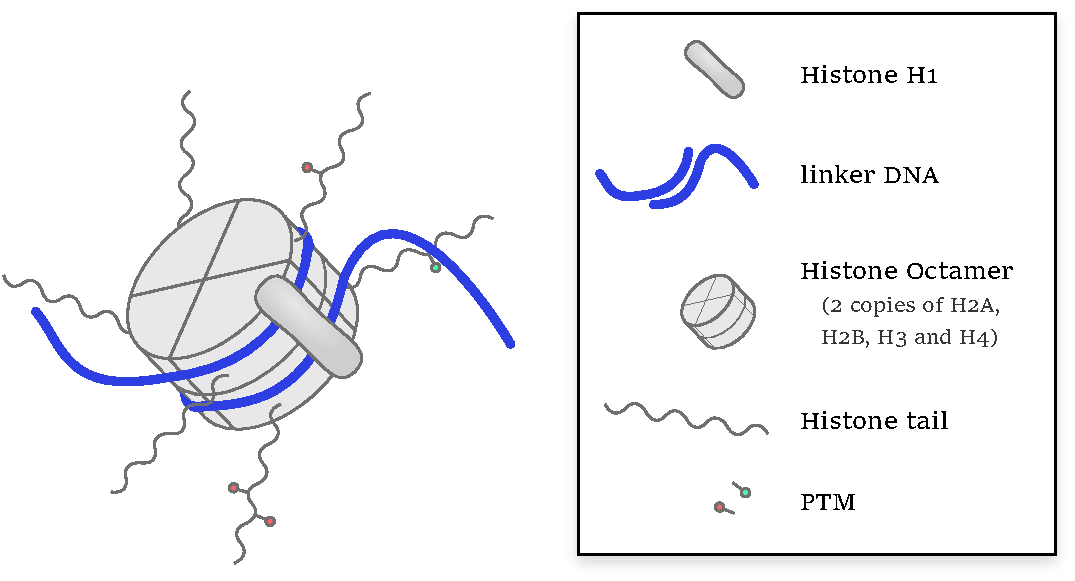
\includegraphics[width=0.7\textwidth]{annotated_nucleosome.pdf}
                \caption{Schematic model of a nucleosome. It consists of DNA wrapped around a histone octamer. The histones themselves are organized as two homologous tetramers (H2A, H2B, H3, H4). The DNA is kept in place by histone H1, which also play a role in establishing higher order chromatin structures.}
                \label{img:nucleosome}
            \end{figure}
            %

            %
            Chromatin can show higher order structure than the simple “beads on a string” variant. As such, nucleosomes that are not necessarily next neighbours along the DNA string can be in near proximity \cite{berg2015stryer}. % TODO The following higher order structures have been found by... % FIXME Source
            %

            %
            Chromatin structure plays an important role in eukaryotic gene expression. Some DNA segments close to and on an actively transcribed gene are more easily accessible by proteins due to a locally more open chromatin structure. These chromatin regions are therefore called hypersensitive sites \cite{cooper2017genome}. Logically, the location of hypersensitive sites depends on the set of active genes and is thus cell-type and age specific \cite{berg2015stryer}.
            %

            %
            The complex process of chromatin remodelling which leads to activation or repression of gene transcription comprises a vast multitude of agents and their inter\-action net\-work is still not fully understood.\\
            %
        %
        %
        \subsection{Histone-modifying enzymes}
            \label{subsec:HME}
            %
            This thesis is based on one aspect of the chromatin remodelling machinery, namely histone-modifying enzyme complexes (HME). These complexes are able to covalently bind or remove chemical groups on amino acids (mostly R and K) at very specific positions on the histone tail. These post-translational modifications (PTMs) are named according to the amino acid they have been bound to. H3K27ac, for instance, denotes an acetylation (ac) on lysine 27 (K27) of histone 3 (H3).
            %

            %
            The presence of these chemical groups changes the charge or polarity of the modified amino acids and thus influences the histone's affinity to the DNA. Histone-acetyl\-transfer\-ases (HATs), for instance, add an acetyl group to lysine, thus neutralizing the positive charge on the ammonium cation at neutral pH (see figure \ref{img:acetyllysineReaction}). This neutralization decreases the attraction to the negatively charged DNA backbone significantly resulting in the occurrence of a hypersensitive site. \cite{berg2015stryer}
            %

            %
            \begin{figure}[htpb]
                \centering
                \vspace{.5cm}
                \schemestart
                    \arrow{0}[,0]
                    \chemname{\chemfig{!{lysine}}}{Lysine}\+\chemname{\chemfig{!{acetylcoa}}}{Acetyl-CoA}
                    \arrow[-90]
                    \chemfig{!{acetyllysine}}\+\chemfig{CoA-SH}\+\chemfig{H^+}
                \schemestop
                \vspace{.5cm}
                \caption{Acetylation of lysine. This reaction is catalysed by the HAT enzyme which by means of the cofactor acetyl coenzyme A (Acetyl-CoA) is able to trigger the transfer (substitution reaction in chemical terms) of an acetyl group onto the nitrogen atom in the side chain of lysine. The latter can be part of a histone tail.}
                \label{img:acetyllysineReaction}
            \end{figure}
            %

            %
            Apart from the acetyl group, a multitude of other markers have been found on histone tails, e.g. methylation (one-, two and three-fold), phosphorylation, ubiquitylation and so forth \cite{bannister2011regulation}. These groups can entail gene transcription activation, silencing (repressing), or fulfil completely different purposes \cite{rossetto2012histone,wang2006histone}. % FIXME source
            %

            %
            The enzymes' modification activities are not forcibly isolated processes. The different enzyme types as well as the modifications on specific amino acids on the histone tails are connected through complex interaction networks \cite{zhang2015interplay, musselman2012perceiving, ge2019nucleation}. Such crosstalk between different modifications is achieved by the enzymes' ability to “read” modifications and “write” another one, if the reading process was successful. Reading is achieved by binding to specific modifications on the histone tail. A very popular example for this behaviour is the bromodomain, which specifically binds acetylated lysines \cite{zeng2002bromodomain}. The modification pattern that certain enzymes need in order to modify an amino acid will further on be called the enzyme's \textit{context}. Upon successful binding, the enzyme can then catalyse the covalent modification of an unmodified amino acid.
            %

            %
            In order to clarify the meaning of the vocabulary concerning the enzyme models, consider the following illustration:
            %

            %
            For the HAT enzyme mentioned earlier, one would define the enzyme’s context as an unmodified nucleosome, as this is needed in order for the enzyme to perform its specific chemical modification reaction on the nucleosome string, which is acetylation of an unmodified nucleosome. Possibly, the enzyme needs a specific reading pattern in order to bind to the string in proximity of the nucleosome to be written on. This is the case when concerning self-reinforcing enzymes, for instance, which read their own modification and are then able to write it to another unmodified nucleosome which results in a positive feedback loop. Such specific reading/binding patterns are also contained in the context of this specific enzyme. Thus, the enzyme’s context is a summary of rules that impose constraints on the presence or absence of modifications on the nucleosome string in order for the enzyme to gain reading/writing ability.\\
            %

            %
            This thesis will only feature acetylation as an activating modification and methylation as a silencing modification. Accordingly, the “state” of a nucleosome is defined as one of the following:
            %

            %
            \begin{itemize}
                \item \textbf{unmodified}: There has been no PTM on any histone tail of the concerning nucleosome.
                \item \textbf{active}: Every PTM found on the concerning nucleosome enables gene activation. In this thesis, every one of these PTMs is an acetylation.
                \item \textbf{silent}: Every PTM found on the concerning nucleosome disables gene activation. In this thesis, every one of these PTMs is a methylation.
                \item \textbf{bivalent}: see \ref{sec:TheoryBivalency}
            \end{itemize}
            %
        %
        %
        \subsection{Bivalency}
            %
            \label{sec:TheoryBivalency}
            In pluripotent stem cells, nucleosomes have been found to contain both activating and silencing markers on histone tails of one and the same octamer. This bivalent state is believed to maintain a “poised state”, being ready to induce a gene expression cascade as soon as the silencing marker is removed \cite{lesch2014poised,bernhart2016changes}. % FIXME source
            Others believe, that this bivalent state is connected to cell division and the ability of inheriting the active gene set for one daughter cell to induce differentiation while the other daughter cell remains a pluripotent stem cell \cite{schuettengruber2017genome}. % TODO is this right?
            %
        %
        %
    %
    %
    \section{Dynamic histone PTM models}
        %
        \subsection{Chemical master equation}
        \label{subsec:CME}
            %
            The chemical master equation (CME) is the differential equation underlying a chemical mixture that describes the time-dependent evolution of said mixture from a reactive point of view. Applied to the case at hand, we can establish the CME system made out of two equations for either the concentration of active (acetylated) and silent (methylated) nucleosome states.
            %

            %
            In order to do this, one can establish the state concentration dependent differential equation \cite{lemons1908paper} for each state type (i.e. active and silent) with respect to the HME types that modify the respective state. This was already done by Mayer in \cite{mayer2020langevin}.
            %

            %
            Eqns. \ref{eqn:noncooperative} describe the non-cooperative (see \ref{subsec:EnzymeTypes}) case for $a = \frac{A}{N}$ and $m = \frac{M}{N}$ with $A$ the number of acetylated nucleosomes, $M$ the number of methylated nucleosomes and $N$ the total number of nucleosomes. $\alpha_i$ and $\beta_i$ are coefficients taking into account the types, association and dissociation ratios of the enzymes in the system. % TODO Referring to correct subsec?
            %

            %
            \begin{subequations}
                \begin{align}
                    &\frac{\partial a}{\partial t} = \underbrace{- \alpha_1 a }_{\textrm{ac removal}} + \underbrace{ \alpha_2 a*(1-a-m) }_{\textrm{ac addition}}\\
                    &\frac{\partial m}{\partial t} = \underbrace{- \beta_1 m }_{\textrm{me removal}} + \underbrace{ \beta_2 m*(1-a-m) }_{\textrm{me addition}}
                \end{align}
                \label{eqn:noncooperative}
            \end{subequations}
            %

            %
            Obviously, this would only be a usable model if the neighbour relations of the nucleosomes could be neglected. Given that the context from the enzyme rule sets is an important aspect of \ed/ (see \ref{subsec:EpiDynast}), an analytical solution of the CME would not be the best approximation. Also, \ed/'s model strongly depends on discrete numbers such as the number of nucleosomes in the string, rendering mere state concentrations without positional information insufficient. Thus, the analytical solution of the CME as a continuous system, makes it even more unfitting as an approximation for the system at hand.
            %

            %
            A more fitting model would be to establish and solve the CME for every nucleosome while the CME for nucleosome $i$ would depend on the number of neighbours equal to the biggest enzyme context in the system's rule set. For instance, if the rule set contains at least one rule including the next neighbours of the modified nucleosome $i$, the CME system would change to eqns. \ref{eqn:neighbourDependent}.
            %

            %
            \begin{subequations}
                \begin{align}
                    &\frac{\partial a_i}{\partial t} = - \alpha_1 (a_{i-1} + a_i + a_{i+1}) + \alpha_2 (a_{i-1} + a_i + a_{i+1})*(1-a-m)\\
                    &\frac{\partial m_i}{\partial t} = - \beta_1 (m_{i-1} + m_i + m_{i+1}) + \beta_2 (m_{i-1} + m_i + m_{i+1})*(1-a-m)
                \end{align}
                \label{eqn:neighbourDependent}
            \end{subequations}
            %

            %
            This differential equation system quickly increases in complexity and dimensionality with increasing number of nucleosomes in the system and higher reach of the enzyme models up to a point where an analytical solution is impossible to achieve. Mainly for this reason, it is convenient to numerically simulate the time-dependent evolution of the system.
            %
        %
        %
        \subsection{Gillespie's algorithm}
        \label{subsec:Gillespie}
            %
            Gillespie's algorithm or \textit{stochastic simulation algorithm}, as called by the author, simulates the evolution in time of a spatially homogenous molecular mixture with a discrete number of reactants under specification of the coupled reaction channels (i.e. association and enzymatic reaction with simultaneous dissociation) based on stochastic chemical kinetics \cite{gillespie1976general, gillespie1992rigorous}. This is useful especially when the practice of solving the chemical master equation analytically is not ideal (see \ref{subsec:CME}).
            %

            %
            Reconsidering the HAT enzyme example from before, its two reaction channels would be the association for one and secondly the reaction and dissociation channel. \\
            %

            %
            Contrarily to other stochastic simulations, Gillespie takes an event-based time step approach. This ensures that at every time step, exactly 1 event is taking place. This approach obviously reduces the overhead compared to an equidistant time step approach (see fig. \ref{img:Gillespie_timeSteps}) and can massively facilitate implementation and later interpretation of the simulation results.
            %

            %
            \begin{figure}[htpb!]
                \centering
                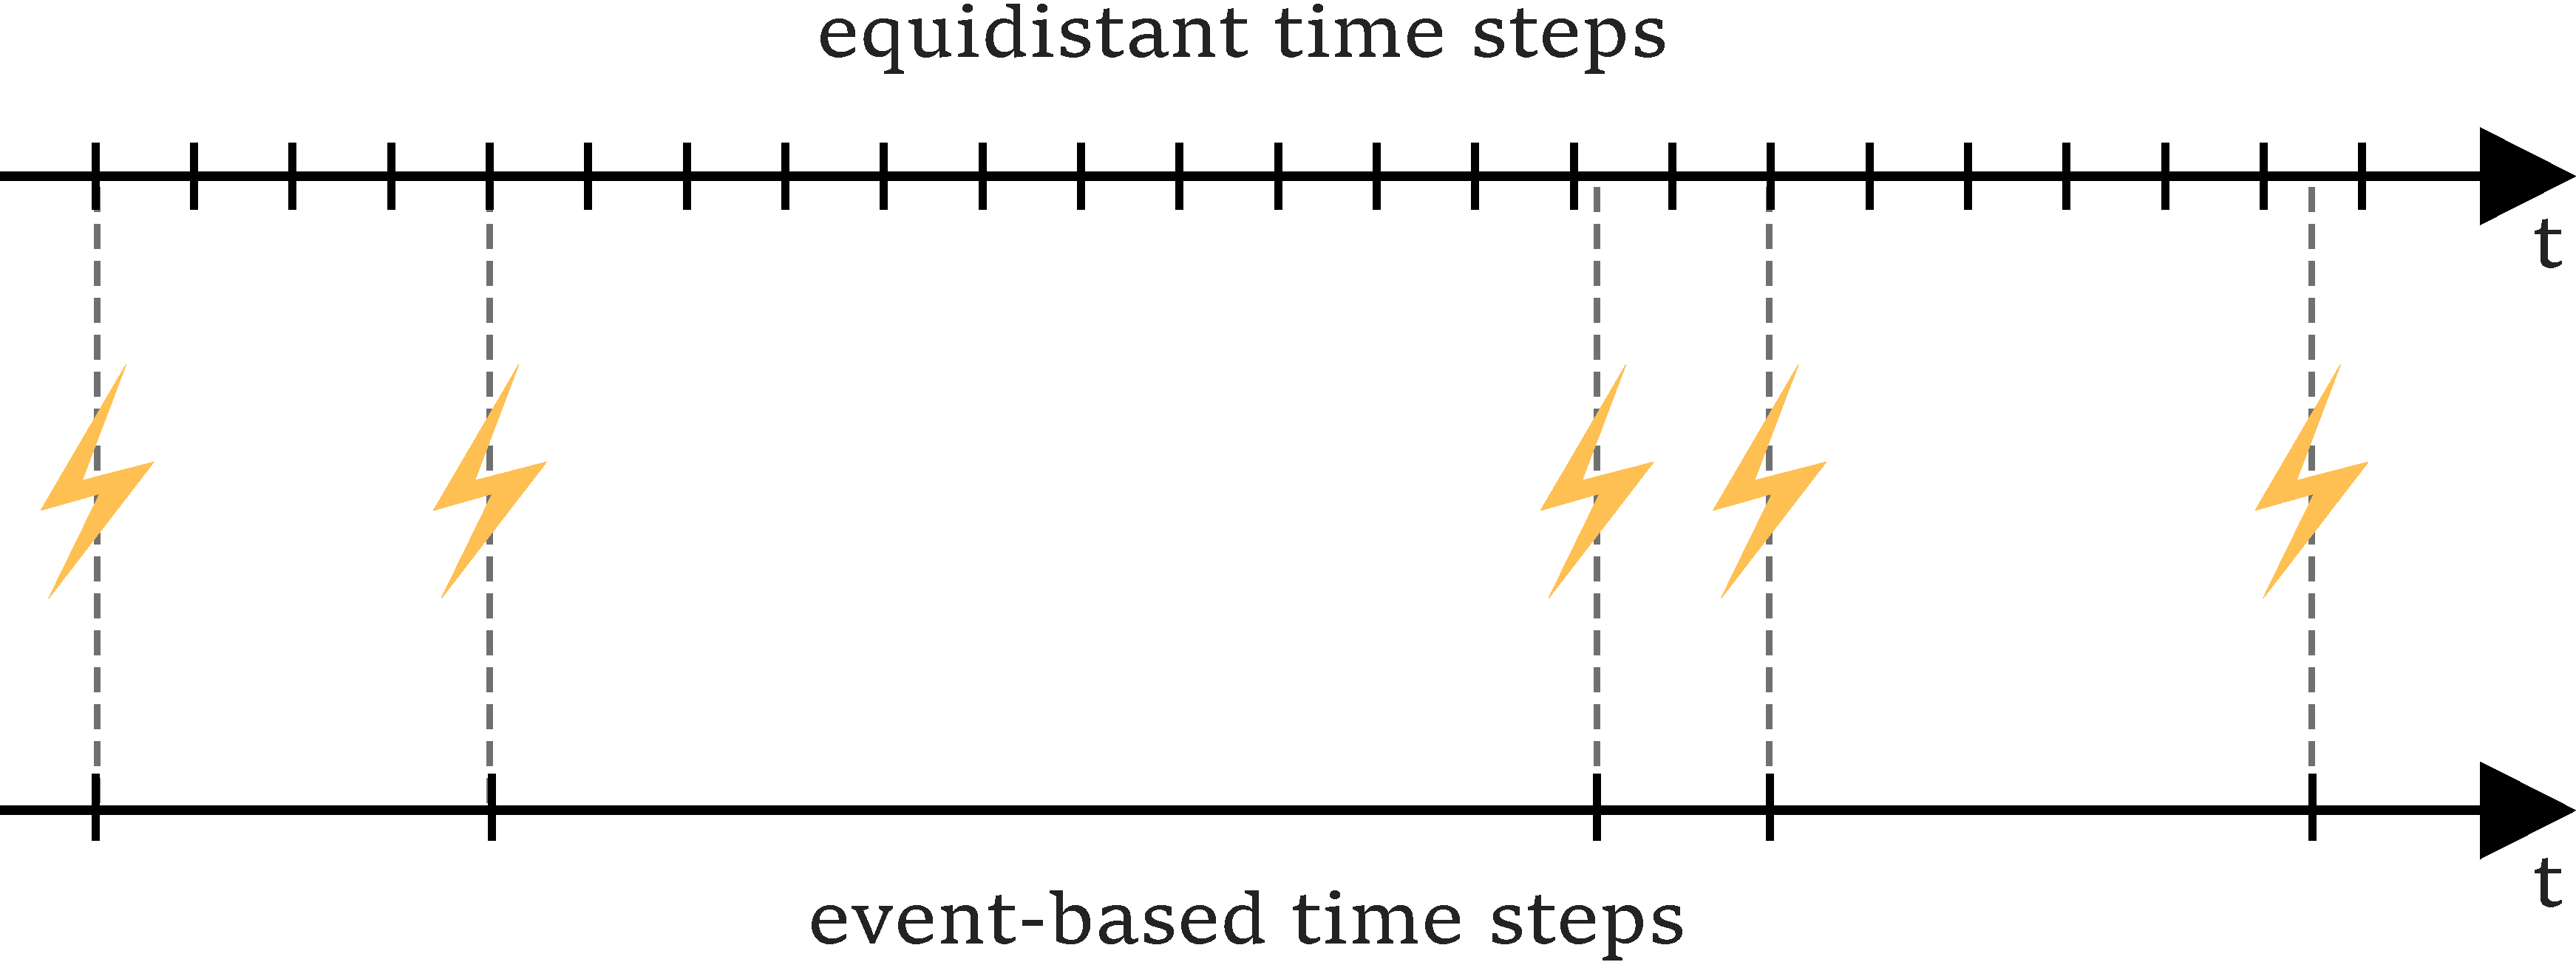
\includegraphics[width=0.7\textwidth]{Gillespie_timeSteps.pdf}
                \caption{Schematic illustration of equidistant time steps vs. event-based time steps inspired by Mayer in \cite{mayer2020langevin}.}
                \label{img:Gillespie_timeSteps}
            \end{figure}
            %

            %
            The algorithm accounts for an appropriate choice of the time elapsed between two time steps by computing and comparing the number of legal associations and dissociations as defined by the enzyme rules given to the algorithm. The rule set in this setting consists of enzymes that covalently modify histone tails. The legality of such a reaction is assessed by checking, if a certain modification pattern (context) is already present on the nucleosome to be modified and other neighbouring nucleosomes on the string in order to perform the reading and writing actions for the specific enzyme.
            %

            %
            The algorithm then summarizes these legal channel possibilities in a propensity sum (normalized from 0 to 1) taking the given association and dissociation rates as well as the concentrations into account. An event is then chosen at random by selecting a random number between 0 and 1. If many events are contributing to the propensity sum at this time step, the time in between events is smaller. Conversely, if only few events are possible at this time step, the time in between events is larger.\\
            %


            %
            In more systematical terms, Gillespie's algorithm can be summarized in the following 4 steps \cite{gillespie1977exact, mayer2020langevin}:
            %

            %
            \begin{itemize}
                \item \textbf{Step 0 (initialization):} Set an initial starting state $X$ and a rule set. Set $t = 0$.
                \item \textbf{Step 1:} Calculate the propensity sum $a_0$ as the sum of all legal reactions and their occurrence possibility based on their association/dissociation rates and their concentration.
                \item \textbf{Step 2:} Based on random numbers, choose a specific reaction channel $\mu$ as the event to happen in this time step as well as the time $\tau$ elapsed from the previous event to the present one.
                \item \textbf{Step 3:} Update the time $t_{i+1} = t_i + \tau$ as well as the effect that $\mu$ has on the system $X_{i+1} = \mu (X_i)$. Continue with step 1.
            \end{itemize}
            %
        %
        %
        \subsection{\ed/}
        \label{subsec:EpiDynast}
            %
            The software used in this thesis is \ed/ (\textbf{Epi}genetic \textbf{Dyna}mics \textbf{S}imulation \textbf{T}ool), which bases on \textit{StoChDyn} by Arnold et al. \cite{arnold2013chromatin} and was developed by N. Herbig et al. (unpublished results).
            %

            %
            \ed/ is a nucleosome post-translational modification (PTM) simulation software which, at its core, uses Gillespie's algorithm in order to show the dynamic change on a nucleosome string as a function of time.
            %

            %
            The main working mechanism may be outlined as follows: First, one defines an enzyme rule set and a starting nucleosome string, which is defined as an array of nucleosomes reduced to their PTMs (see \ref{sec:ChromatinModel}). Then, \ed/ simulates the stochastic time-dependent change of said modifications on the string, exactly one event at a time. The two events that can occur for each enzyme are either an association step or a reaction step that immediately entails the enzyme's dissociation from the nucleosome.
            %

            %
            The enzyme rule sets simply describe a pattern (further on called “context” % TODO is the context including the site that is changed? Context is already explained at Gillespie
            ) on the string, that is then changed according to the rule. For instance, a linear acetylation extender enzyme would look for a pattern with two neighbouring nucleosomes, one acetylated and the other one unmodified, and acetylate the latter (see \ref{subsec:EnzymeTypes} for details on the enzyme types and their reactions).
            %
        %
        %

    %
    %
    \section{Epigenetic fitness landscapes} % TODO change title
        %
        \subsection{From landscape to vector field}
            %
            The term of fitness landscape (referred to as landscape for the rest of this work) is mathematically defined as the triple $(V, \chi, f)$ where $V$ is a set of configurations, $\chi$ refers to the neighbouring relationship or similarity among the configurations and $f$ defines the fitness function of the landscape \cite{Stadler2002} (see fig. \ref{img:fitnessLandscape} for a simplified example).
            %

            %
            In the case of epigenetic fitness landscapes, $V$ comprises the entirety of active, silent and unmodified state distributions along the nucleosome string, $\chi$ determines the dissimilarity between two nucleosome strings, i.e. which nucleosome has to be changed on the string $v_1 \in V$ in order to turn it into another nucleosome string $v_2$. $f$, which indicates the relative height or depth $f(v)$ of a specific configuration $v \in V$, is determined by all the association and dissociation rates, as well as the type of the enzymes in the system. In this specific landscape, the stochastic Gillespie's algorithm will always tend towards configurations (fix points) at the very base of landscape basins. These configurations are those, that are adopted in the majority of time steps throughout Gillespie's simulation algorithm.\\ % TODO chi as a measure of distance thus usable in definition of bistability
            %

            %
            The term of epigenetic fitness landscape defined in this work is not to be confounded with the very frequently referenced concept of “epigenetic landscape” introduced by C. H. Waddington around 1957 \cite{waddington2014strategy}. The epigenetic landscape describes a conceptual model which draws an analogy between cell differentiation with its influential factors and a ball on a rugged hill \cite{epilandscapeDefEmbryo}. The ball inevitably rolls down the hill, but the exact track it is taking along its way down will fundamentally decide, where it is going to end up in the valley. Analogously, the observed cell's fate will eventually be differentiation, but, according to Waddington, the pathway taken along the branched track is defined by the starting point, gene interaction (regulation) and the counterplay of inductive events, which push the cell in a distinct direction on the landscape, and the cell's competence or ability to follow this path.
            %

            %
            \begin{figure}[!htpb]
                \centering
                \begin{minipage}[t]{\textwidth}
                    \begin{minipage}{0.19\textwidth}
                        \caption*{\small \textbf{(a)}}
                    \end{minipage}
                    \begin{minipage}{0.8\textwidth}
                        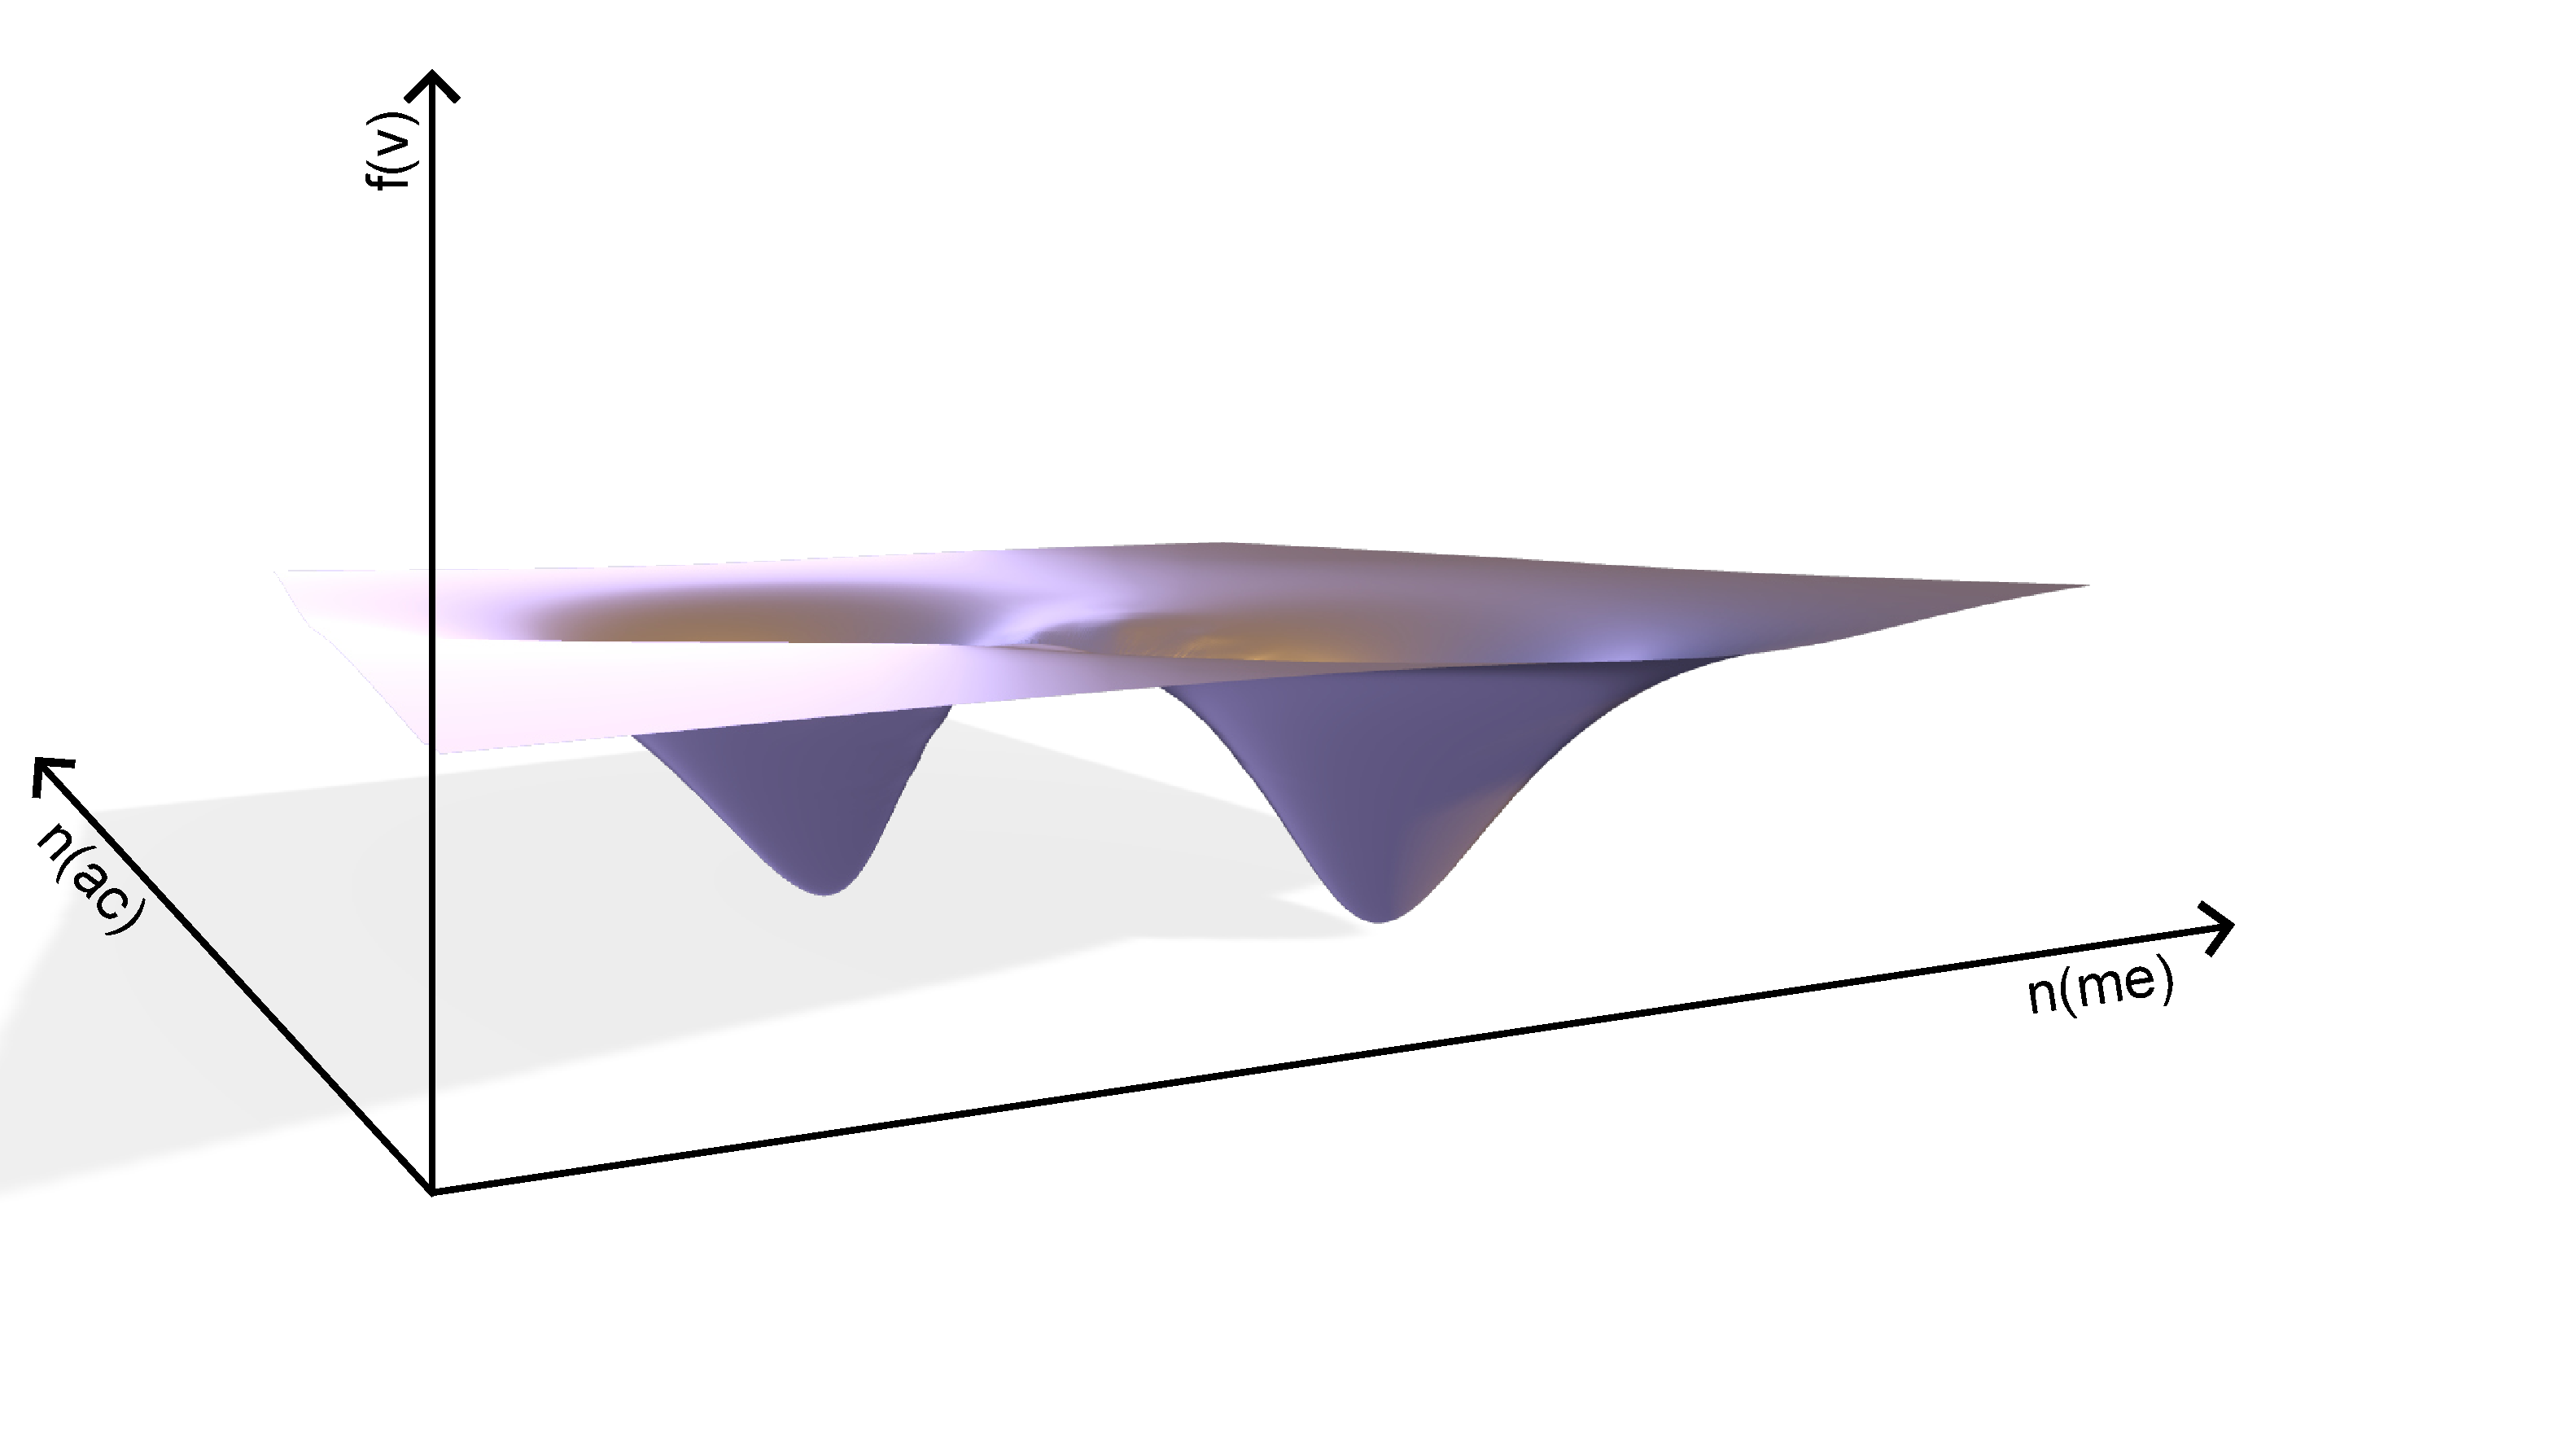
\includegraphics[width=\textwidth]{landscape_wAxes.pdf}
                    \end{minipage}
                    \begin{minipage}{0.19\textwidth}
                        \caption*{\small \textbf{(b)}}
                    \end{minipage}
                    \begin{minipage}{0.8\textwidth}
                        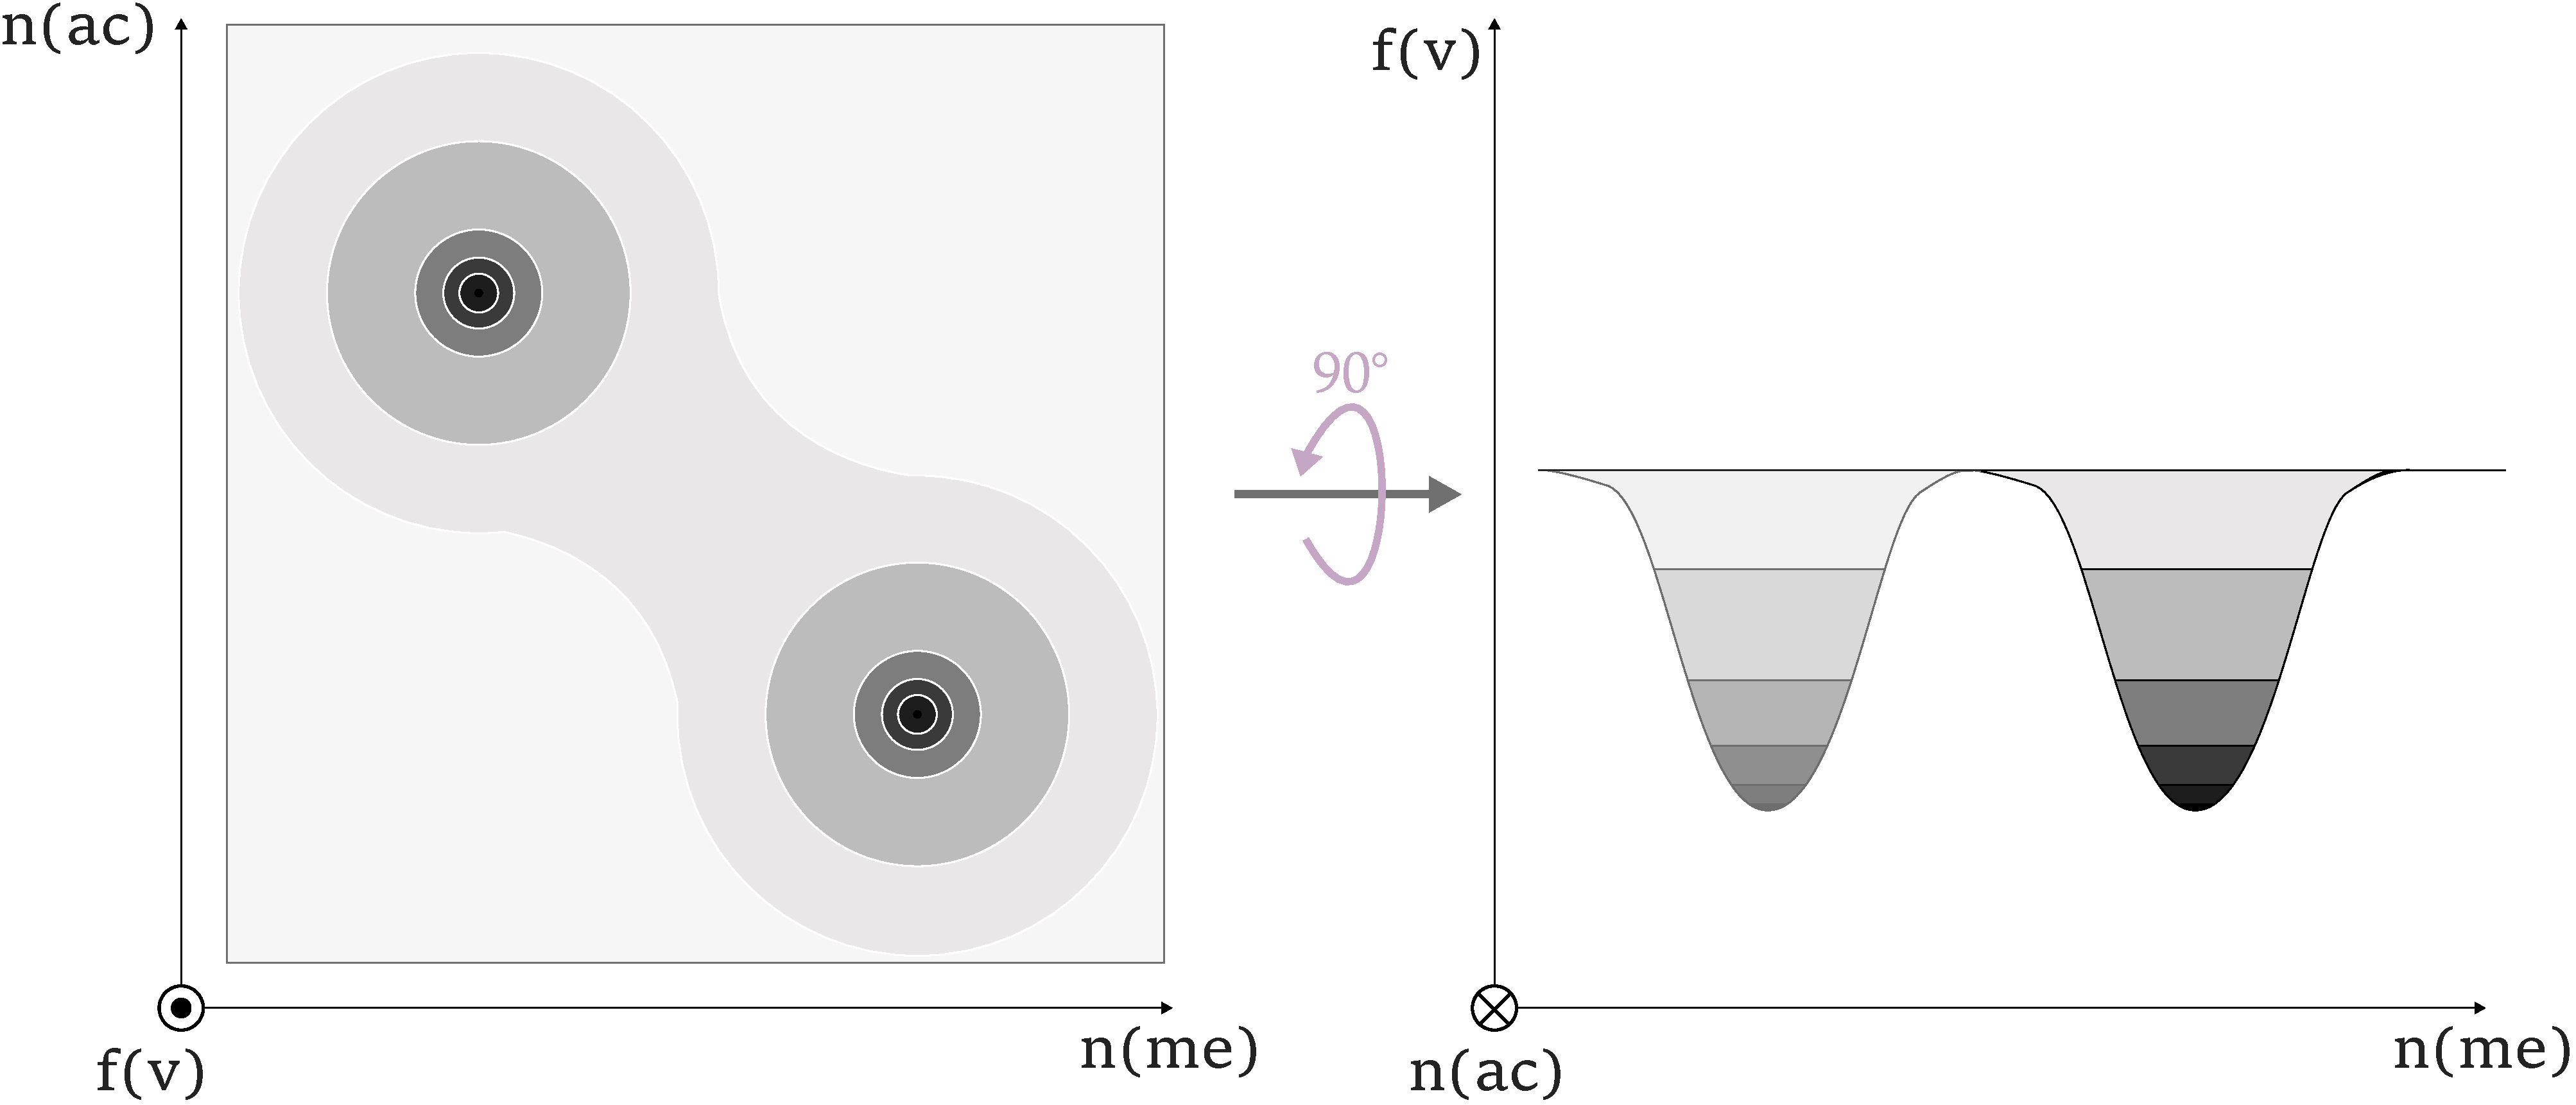
\includegraphics[width=\textwidth]{landscape_wAxes_2D.pdf}
                    \end{minipage}
                \end{minipage}
                \caption{Simplified epigenetic fitness landscape example of a bistable system. \textbf{(a)} 3D illustration modelled with Blender \cite{blender}. \textbf{(b)} 2D-projections along the indicated axes. The fix points in the basins are the most frequent configuration throughout a simulation. In most bistable systems, the basins are to be found at the extrema of the $n(ac)$ and the $n(me)$ axes.}
                \label{img:fitnessLandscape}
            \end{figure}
            %

            %
            The idea of landscapes is very similar in the concept of Waddington's cell differentiation model as well as in the epigenetic fitness landscape model used in this work. However, the underlying phenomenon that is explained is entirely different. Waddington aims at providing a graspable model for a stem cell's journey through differentiation. The epigenetic fitness landscape model defined in this work however serves the purpose of explaining histone PTMs on a chromatin string. Furthermore, the fitness landscape is a mathematically graspable concept with numerical influential factors and a slope defined by $f$ while Waddington's model only offers a figurative model.
            % TODO Include? Another important difference is that Waddington's ball will end up on the bottom of the hill while the chromatin string can exit a basin again.
            % TODO Is a fix point the end?
            %

            %
            Nonetheless, in order to avoid confusion on the reader's side, Waddington's definition of the epigenetic landscape will not be featured from this point on in this work. Every mention of landscape will refer to the epigenetic fitness landscape mathematically defined above.
            %

            %
            Depending on the landscape, i.e. if there are deep and steep basins, it gets more and more difficult for the system to exit the basin and adopt a configuration that lies outside. Each histone modifying enzyme thus induces an individual stability trend among the configurations which results in a vector field specific to each type of enzyme. In more complex systems with a multitude of different enzyme types, these vector fields are combined by superposition and create the resulting landscape at hand containing zero or more fix points, depending on the un-, mono- or multistable nature of the system.
            %

            %
            In this thesis,  there won't be any numerical values given to $f(v)$. However, by modifying the relative enzyme rate ratios, one can easily see that $f$ can change drastically resulting in variation of ease for the system to maintain a certain state or move along the shape of the landscape to switch from one state to another. Thus, even though $f$ can not be numerically anchored, the influential factors that change $f(v)$ for one $v \in V$ as well as their impact on the landscape can very well be identified.
            %
        %
        %
        \subsection{Monostable landscapes}
        \label{subsec:monostability}
            %
            The number of fix points in the landscape can be analytically derived from the differential equation system that can be established for a given set of enzyme types.
            %

            %
            \begin{figure}[!htbp]
                \centering
                \begin{minipage}{0.3\textwidth}
                    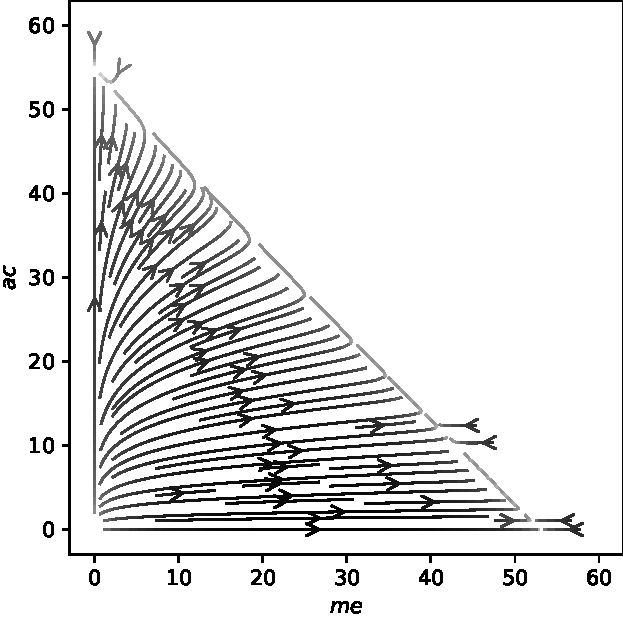
\includegraphics[width=\textwidth]{vectorfield_noncooperative_assymetric_monostable_ac.pdf}
                    \caption*{\small \textbf{(a)}}
                \end{minipage}
                \begin{minipage}{0.3\textwidth}
                    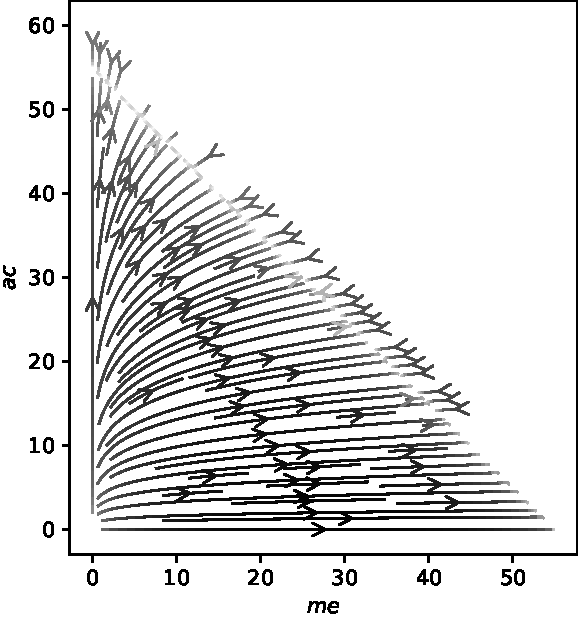
\includegraphics[width=\textwidth]{vectorfield_noncooperative_asymmetric_multistable.pdf}
                    \caption*{\small \textbf{(b)}}
                \end{minipage}
                \begin{minipage}{0.3\textwidth}
                    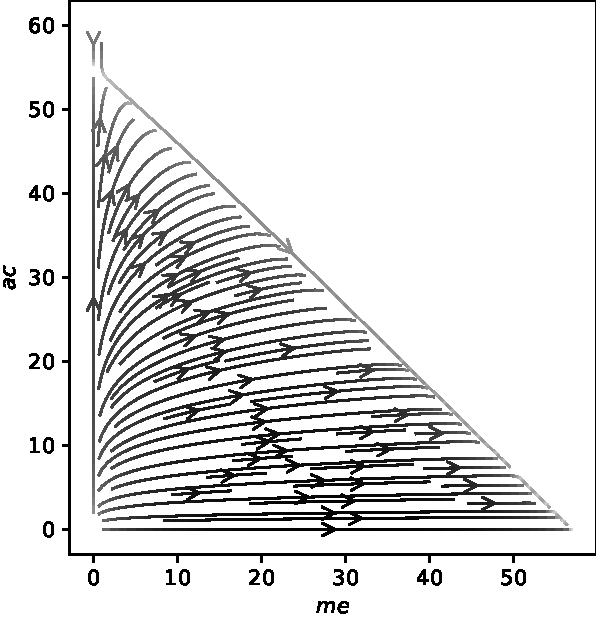
\includegraphics[width=\textwidth]{vectorfield_noncooperative_assymetric_monostable_me.pdf}
                    \caption*{\small \textbf{(c)}}
                \end{minipage}
               \caption{Vector fields describing the non-cooperative 60 nucleosome system with varying enzyme rates. These mainly define the parameters $\alpha_n$ and $\beta_n$ if the enzyme types are constant. The axes describe in absolute numbers the occurrence of methylation (x-axis) and acetylation (y-axis). \textbf{(a)} describes the case for $\frac{\alpha_1}{\alpha_2} > \frac{\beta_1}{\beta_2}$ resulting in a separatrix with gradient towards $(0,N(1-\frac{\beta_1}{\beta_2}))$. In \textbf{(b)}, the equality $\frac{\alpha_1}{\alpha_2} = \frac{\beta_1}{\beta_2}$ results in a zero-gradient separatrix. In \textbf{(c)}, $\frac{\alpha_1}{\alpha_2} < \frac{\beta_1}{\beta_2}$ results in a separatrix with gradient towards $(N(1-\frac{\alpha_1}{\alpha_2}),0)$. From Mayer in \cite{mayer2020langevin}.}
               \label{img:nonCooperativeVectorFields}
            \end{figure}
            %

            %
            In \cite{mayer2020langevin}, Mayer found 4 critical values for eqns. \ref{eqn:noncooperative} in the Cartesian coordinate system $(m,a)$ with origin $(0,0)$ and $m$ the amount of methylated nucleosomes and $a$ the amount of acetylated nucleosomes. 3 are fix points at $(0,0)$, $(0,1-\frac{\beta_1}{\beta_2})$, $(1-\frac{\alpha_1}{\alpha_2},0)$ and one is a separatrix whose gradient depends on the ratio between $\frac{\alpha_1}{\alpha_2}$ and $\frac{\beta_1}{\beta_2}$ and which connects the two non-trivial fix points. The separatrix always has a gradient towards one of the non-trivial fix points, except for the case $\frac{\alpha_1}{\alpha_2} = \frac{\beta_1}{\beta_2}$. Here, the separatrix has no gradient (see fig.\ref{img:nonCooperativeVectorFields}).
            %

            %
            One could argue, that for the case of $\frac{\alpha_1}{\alpha_2} = \frac{\beta_1}{\beta_2}$, the zero-gradient separatrix interpreted as a set of points fulfilling a linear equation presents an infinite amount of stable points, thus rendering this specific system multistable. However, one point on the separatrix can hardly be described stable, because it is not resistant to small perturbations. In fact, even the most atomic displacement defined in the system by $\chi$, namely the state change of one nucleosome, most likely leads to another point on the separatrix and not forcibly to the previous one. Thus, the separatrix as a whole, containing both non-trivial fix points can be described as stable and disqualifies every other point on the separatrix from individual stability, hence the monostable nature of all the systems in fig. \ref{img:nonCooperativeVectorFields}.
            %


            \subsection{Multistable landscapes}
            %
            In order for a dynamic histone PTM system to be bistable, the enzymes have to show cooperativity \cite{dodd2011barriers,sneppen2019theoretical,mayer2020langevin}. According to Sneppen \cite[][p.48]{sneppen2014models}, \enquote{cooperative binding means that the probability of occupying a state increases more than linearly with the concentrations of the binding molecules}.
            %

            %
            In \cite{dodd2011barriers}, Dodd et al. specify the nature of cooperativity in order to reach ultrasensitivity\footnote{From Dodd et al. \cite{dodd2011barriers}: \enquote{Ultrasensitivity is a nonlinearity that magnifies any numerical advantage of one nucleosome type over another, allowing positive feedback to strongly push the system away from intermediate states and towards a large majority of one or other type.}} and thus a bistable system as follows\footnote{citations inside the quote changed their appearance in order to remain functional and to stylistically fit this work}:
            %

            %
            \begin{quote}
                “Cooperativity can be direct, where two modified nucleosomes act together to recruit an enzyme to modify a third nucleosome \cite{3dodd2007theoretical,11sedighi2007epigenetic,15micheelsen2010theory}, or indirect, where each modified nucleosome catalyzes one of two separate modification reactions to fully convert a third nucleosome \cite{3dodd2007theoretical,13david2009inheritance}. A critical requirement for ultrasensitivity is that modified nucleosomes must act nonlocally, stimulating modification of nucleosomes located some distance away on the DNA. This long-range interaction is necessary for any nucleosome to be able to ‘sense’ the majority nucleosome type within the patch and cannot be provided by simple neighbor-to-neighbor contact \cite{3dodd2007theoretical,15micheelsen2010theory}.”
            \end{quote}
            %

            %
            In other words, cooperativity can only be achieved by allowing the enzymes to detect more than one nucleosome that, in order to reach bistability, must not be a direct neighbour of the nucleosome to be (un)modified. This allows the modification that is superiorly prevalent over the whole string at that moment to be accounted for and recognized by the enzymes.\\
            %

            %
            On a sidenote, the definition of cooperativity might seem slightly counterintuitive from a biochemical point of view, where the notion of cooperativity is strongly associated to be an asset of the enzyme \cite{cooperativityDefBritannica}. In contrast, according to Dodd et al., cooperativity is described as being a property of a set of nucleosomes being able to “cooperate” in order to recruit an enzyme and catalyse a reaction. A biochemist might be more comfortable with the enzymes being the active part in the system and most notably the catalyst of the occurring reactions instead of the nucleosomes, which most definitely do not catalyse any chemical reaction.
            %

            %
            Even though this is not ideally put from a biochemical point of view, the mathematical implications are untouched from these imprecisions.\\
            %

            %
            Mayer in \cite{mayer2020langevin} expressed the time dependent concentration of the modifications in the system in function of cooperative enzymes in the differential equation system in eqns. \ref{eqn:cooperative}.
            %

            %
            \begin{subequations}
                \begin{align}
                    &\frac{\partial a}{\partial t} = \underbrace{- \alpha_1 a }_{\textrm{ac rem}} + \underbrace{ \alpha_2 \frac{1}{n} a^2*(n-a-m) }_{\textrm{ac add}}\\
                    &\frac{\partial m}{\partial t} = \underbrace{- \beta_1 m }_{\textrm{me rem}} + \underbrace{ \beta_2 \frac{1}{n} m^2*(n-a-m) }_{\textrm{me add}}
                \end{align}
                \label{eqn:cooperative}
            \end{subequations}
            %

            %
            Given that the cubic cooperative terms show the highest potency, it is known that the differential equation system has a maximum of 9 critical values. Some of these critical values can quite easily identified graphically.
            %

            %
            Fig. \ref{img:cooperativeVectorField} depicts the vector field of a system with random and cooperative enzymes. Some critical values can clearly be identified. They are summarized in tab. \ref{tab:cooperativeCriticalValues}.
            %

            %
            \begin{figure}[htbp!]
                \centering
                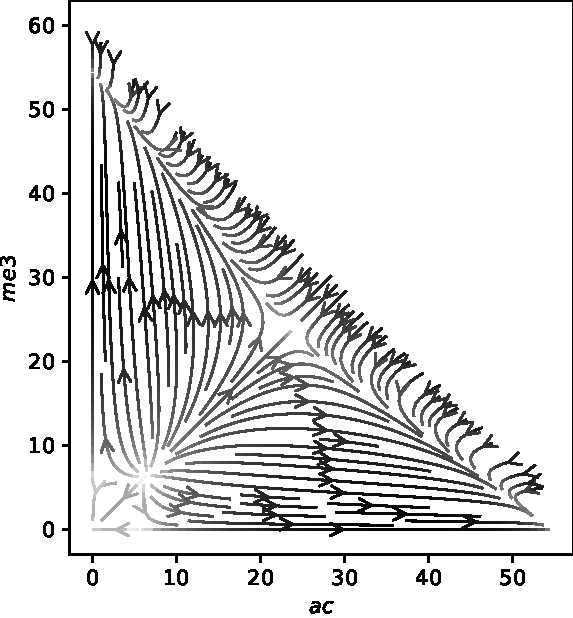
\includegraphics[width=.5\textwidth]{vectorfield_cooperative.pdf}
                \caption{Vector fields describing the cooperative 60 nucleosome system with varying enzyme rates. These mainly define the parameters $\alpha_n$ and $\beta_n$ if the enzyme types are constant. The axes describe in absolute numbers the occurrence of methylation (x-axis) and acetylation (y-axis). From \cite{mayer2020langevin}.}
                \label{img:cooperativeVectorField}
            \end{figure}
            %

            %
            \begin{table}[htbp!]
                \caption{Critical values in $(a,m)$ notation as identified graphically in fig. \ref{img:cooperativeVectorField}.}
                \begin{center}
                    \begin{tabular}{l r}
                        \hline
                        \textbf{critical point} & \textbf{stability} \\
                        \hline
                        $(0,0)$     & stable \\
                        $(8,8)$     & unstable \\
                        $(0,5)$     & unstable \\
                        $(5,0)$     & unstable \\
                        $(0,55)$    & stable \\
                        $(55,0)$    & stable \\
                        $(25,25)$   & saddle point \\
                        \hline
                    \end{tabular}
                \end{center}
                \label{tab:cooperativeCriticalValues}
            \end{table}
            %
        %
        %
    %
    %
    \section{Impact of this work}
        %
        Although the mathematical foundation on whether a system can and cannot show bistability was already established, the execution in terms of building a model and rigorously identifying the influence of different factors within the model on the dynamics of a bistable system have, to my knowledge, not been explored yet.
        %

        %
        Also, to date, bistable systems have not yet been modelled by means of a software that takes limited enzyme reach into account like \ed/ does. This is an important distinction from other models, because neighbour-to-neighbour relations are not neglected, which marks an important step towards real-life chromatin systems.\\
        %

        %
        This thesis will show the potential and limitations of a model with fixed neighbour relations concerning bistability and the switching of stable states throughout the simulation. Furthermore, this work will propose working mechanisms of bistability occurring on non-cyclic, as well as cyclic nucleosome strings.
        %
    %
    %
%
%
